\section{Refinement of Symbolic Value Analysis + Constraints CPA}

\begin{figure}[h!]
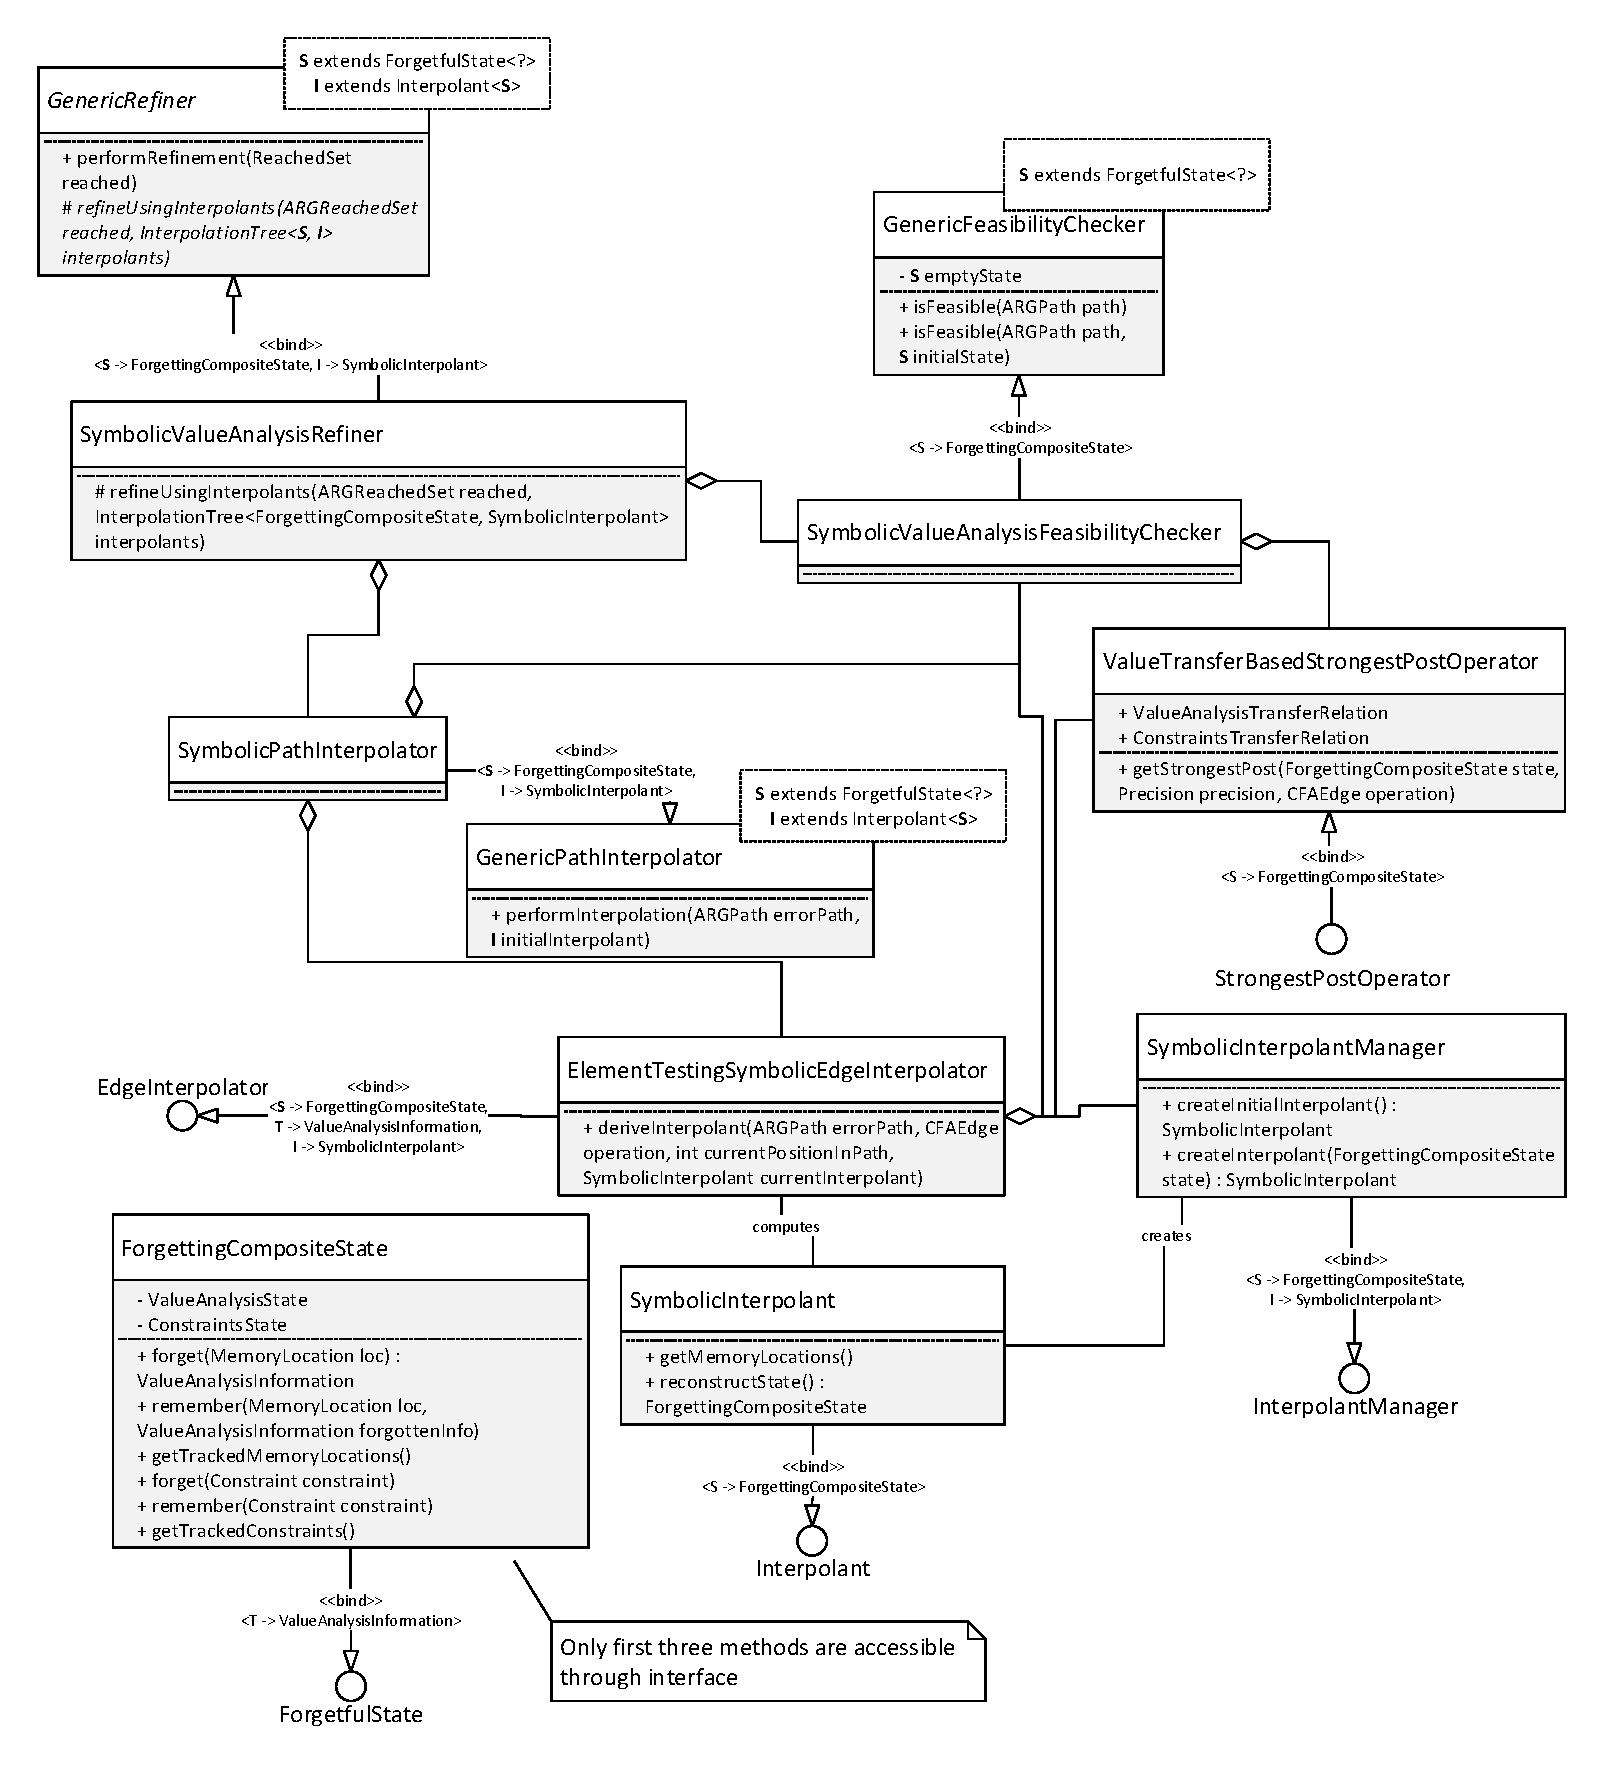
\includegraphics[width=\linewidth]{implementationCegar/RefinementSymEx}
\caption{Structure of refinement procedure for symbolic execution}
\label{fig:refSymbolic}
\end{figure}
Refinement of the \symbolicValueAnalysisCPA\ and \constraintsCPA\ is strongly based on these generic implementations.
Besides \objectName{Interpolant}, \objectName{ForgetfulState}, \objectName{InterpolantManager} and \objectName{StrongestPostOperator}, we only
create an own implementation of \objectName{EdgeInterpolator}.
For all other components, we inherit the behaviour of the generic implementations.
Figure~\ref{fig:refSymbolic} shows the structure of this refinement.

\objectName{Sym\-bo\-lic\-Inter\-po\-lant} implements \objectName{Interpolant}.
It stores information about abstract variable assignments and constraints, so it can be used for interpolating over both these types.
\objectName{Forget\-ting\-Com\-po\-site\-State} implements \objectName{ForgetfulState}.
It is the composition of \objectName{ValueAnalysisState} and \objectName{ConstraintsState} and provides methods for forgetting/remembering both their elements separately.
This is necessary for interpolation, described below.
\objectName{SymbolicInterpolantManager} is an \objectName{InterpolantManager} able to create \objectName{SymbolicInterpolants}.
\objectName{Value\-Trans\-fer\-Based\-Strong\-est\-Post\-Operator} is the implementation of the composite strongest-post operator using the value analysis transfer relation and constraints transfer relation,
described in Section~\ref{sec:assignmentRefinement}.

\objectName{Sym\-bo\-lic\-Edge\-Inter\-po\-lator} implements \objectName{EdgeInterpolator}.
We can't use the functionality of \objectName{Generic\-Edge\-Inter\-po\-lator} since, depending on the configuration, we have to interpolate
testing both constraints and/or variable assignments for their necessity.
The generic edge interpolator only tests program variables (\objectName{Me\-mo\-ry\-Lo\-cations}), though.

\subsection{Optimization: Perform basic value analysis refinement first}
The strongest-post operator $\strongestPostOpSym$ of symbolic execution refinement performs a SAT check at every assume operation, just like the \symbolicExecutionCPA's transfer relation.
To minimize these expensive computations, we refine using the semantics of value analysis's strongest-post operator $\strongestPostOpExplicit$ only, if possible.
To do this, we can't just use value analysis refinement because of the wrong interpolant type of $\Gamma$ and the different precision type.
If value analysis refinement was to update the precision by taking the current precisions of the locations whose states were removed from the reached set after successful interpolation and combining them with the newly computed precision, it would only consider the precision of the \valueAnalysisCPA\ and discard the existing precision of the \constraintsCPA.
So instead, we built a new refinement procedure with a strongest-post operator representing the semantics of $\strongestPostOpExplicit$ (see Section \ref{sec:assignmentRefinement}),  generic refinement classes for interpolation and feasibility check using this strongest-post operator and \objectName{ForgettingCompositeState}, as well as \objectName{SymbolicValueAnalysisRefiner}, which considers the precisions of both \valueAnalysisCPA\ and \constraintsCPA.

\begin{figure}[t!]
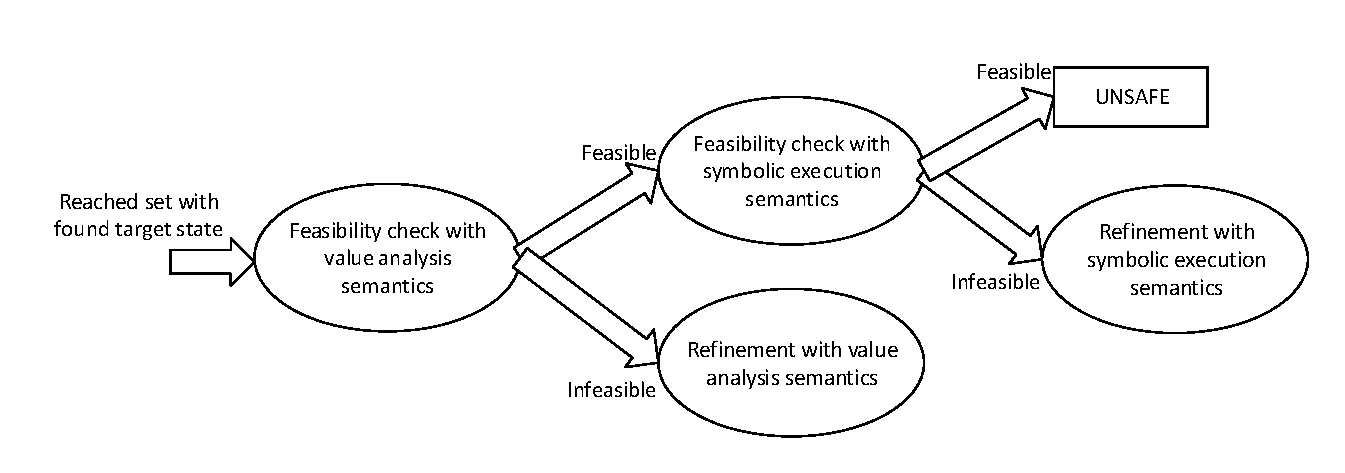
\includegraphics[width=\linewidth]{implementationCegar/DelegatingRefinementFlow}
\caption{Symbolic execution refinement procedure. Before using constraints, try to prove infeasibility with value analysis semantics only}
\label{fig:delegatingRefFlow}
\end{figure}
When refining, we first call this procedure. If it is able to prove the error path as infeasible, we use its refined precision.
If it can't, we use our refinement procedure for symbolic execution to get a new precision.
This way we only use SAT checks in refinement and only increase the precision of the expensive \constraintsCPA\ if this is really necessary for computing an error path as infeasible.

%\subsubsection{Optimization: Different Precision Types}
It is possible to choose the precision type to use for the \constraintsCPA\ with configuration property \configOption{cpa.constraints.refinement.precisionType}.
Possible values are \configOption{CONSTRAINTS} and \configOption{LOCATION} for the corresponding types.

\subsection{Extract precision from predicate refinement}
For using the refinement procedure extracting a precision from the predicate precision created by \predicateCPA's refinement, \predicateCPA's refinement is just executed
and all program variables are extracted from the predicates of the resulting precision for each location.
These program variables are then used for the precision of the \valueAnalysisCPA, while the locations are used as precision for the \constraintsCPA, since it is not possible to derive an original assume statement from the predicates created by \predicateCPA's refinement.
Since the \predicateCPA is more powerful than the \symbolicExecutionCPA, it is possible that a refined precision is returned that is not sufficient for the \symbolicExecutionCPA\ to prove the infeasibility of the error path.
Because of this it is not always possible to use this alternative.
